\begin{figure}[htbp]\centering
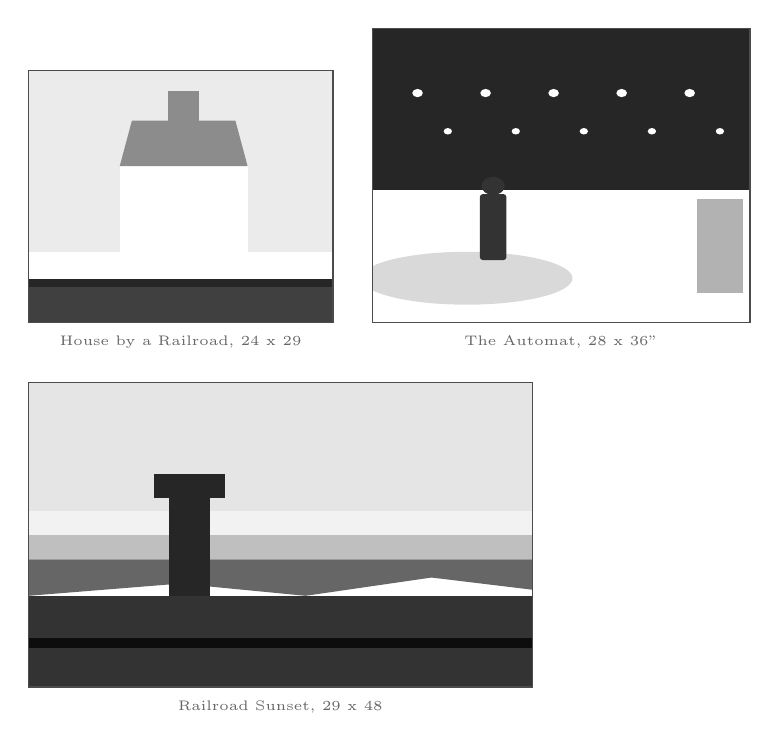
\begin{tikzpicture}
\begin{scope}[shift={(0,0)},x=3.867cm,y=3.200cm]\clip (0,0) rectangle (1,1);
\fill[black!8] (0,0.28) rectangle (1,1);            % sky
\fill[black!75] (0,0) rectangle (1,0.14);           % the embankment and rail
\fill[black!85] (0,0.14) rectangle (1,0.17);
\fill[white] (0.3,0.17) rectangle (0.72,0.62);      % the house
\fill[black!45] (0.3,0.62) -- (0.72,0.62) -- (0.68,0.8) -- (0.34,0.8) -- cycle; % mansard
\fill[black!45] (0.46,0.8) rectangle (0.56,0.92);   % the tower
\end{scope}
\draw[black!70,line width=0.5pt] (0,0) rectangle (3.8666666666666667,3.2);
\node[anchor=north,font=\tiny,text=black!60] at (1.9333333333333333,-0.05) {House by a Railroad, 24 x 29};
\begin{scope}[shift={(4.366666666666667,0)},x=4.800cm,y=3.733cm]\clip (0,0) rectangle (1,1);
\fill[black!85] (0,0.45) rectangle (1,1);            % the window, night
\foreach \x in {0.12,0.3,0.48,0.66,0.84} \fill[white] (\x,0.78) circle (0.014);
\foreach \x in {0.2,0.38,0.56,0.74,0.92} \fill[white] (\x,0.65) circle (0.011);
\fill[black!15] (0.25,0.15) ellipse (0.28 and 0.09); % table
\fill[black!80] (0.32,0.46399999999999997) circle (0.030799999999999998); \fill[black!80,rounded corners=1pt] (0.28500000000000003,0.21200000000000002) rectangle (0.355,0.436);
\fill[black!30] (0.86,0.1) rectangle (0.98,0.42);   % radiator
\end{scope}
\draw[black!70,line width=0.5pt] (4.366666666666667,0) rectangle (9.166666666666668,3.7333333333333334);
\node[anchor=north,font=\tiny,text=black!60] at (6.7666666666666675,-0.05) {The Automat, 28 x 36"};
\begin{scope}[shift={(0,-4.633333333333334)},x=6.400cm,y=3.867cm]\clip (0,0) rectangle (1,1);
\fill[black!10] (0,0.42) rectangle (1,1);          % sky, the sunset in bands
\fill[black!25] (0,0.42) rectangle (1,0.5);
\fill[black!5] (0,0.5) rectangle (1,0.58);
\fill[black!60] (0,0.3) -- (0.3,0.34) -- (0.55,0.3) -- (0.8,0.36) -- (1,0.32) -- (1,0.42) -- (0,0.42) -- cycle; % the dark hills
\fill[black!80] (0,0) rectangle (1,0.3);            % the embankment
\fill[black!95] (0,0.13) rectangle (1,0.16);        % the rails
\fill[black!85] (0.28,0.3) rectangle (0.36,0.62);   % the signal tower
\fill[black!85] (0.25,0.62) rectangle (0.39,0.7);
\end{scope}
\draw[black!70,line width=0.5pt] (0,-4.633333333333334) rectangle (6.4,-0.766666666666667);
\node[anchor=north,font=\tiny,text=black!60] at (3.2,-4.683333333333334) {Railroad Sunset, 29 x 48};
\end{tikzpicture}
\caption{\textbf{House by a Railroad}, oil, 1925; catalogued as House by the Railroad, 24 x 29 as the leaf writes it (Book I, leaf 52, ref 18056). The Museum of Modern Art, 3.1930: \url{https://www.moma.org/collection/works/78330}. \textbf{The Automat}, oil, 1927, 28 x 36" as the leaf writes it (Book I, leaf 54; Dealers, leaf 56). Des Moines Art Center, 1958.2: \url{https://desmoinesartcenter.org/wp-content/uploads/2022/04/cc-hopper.pdf}. \textbf{Railroad Sunset}, oil, 1929; « A real beauty this one. », 29 x 48 as the leaf writes it (Book I, leaf 58, ref 18297). Whitney Museum of American Art, work 5874: \url{https://whitney.org/collection/works/5874}. Scale: sixty inches to eight centimetres, the scale of every canvas frame in this note. The drawings are schemas of the composition in its main masses only, at the proportions of the size in Edward Hopper's hand, made from the leaf's description and from general knowledge of the picture; nothing is traced and no detail is drawn, and they are not reproductions. The pictures themselves are at the museums' own pages. Drawn by Claude Fable~5.1, 13 September 2026, from the transcriptions and \texttt{works.json} (2026-09-13).}\label{fig:bookioils}
\end{figure}
